\subsection{Models}
This section shows the methods to obtain a model trained on HHG images, diagnoses and clinical context.
The final model, a combination of two models together named SCLICOM (from Self-supervised pre-training and CLInical COntext-aware Multi-instance learning), should be able to explain itself via attention maps, which are compared with pathologist annotations.
The pipeline is summarized in \cref{fig:flowchart-sclicom}.

\begin{figure*}
    \centering
    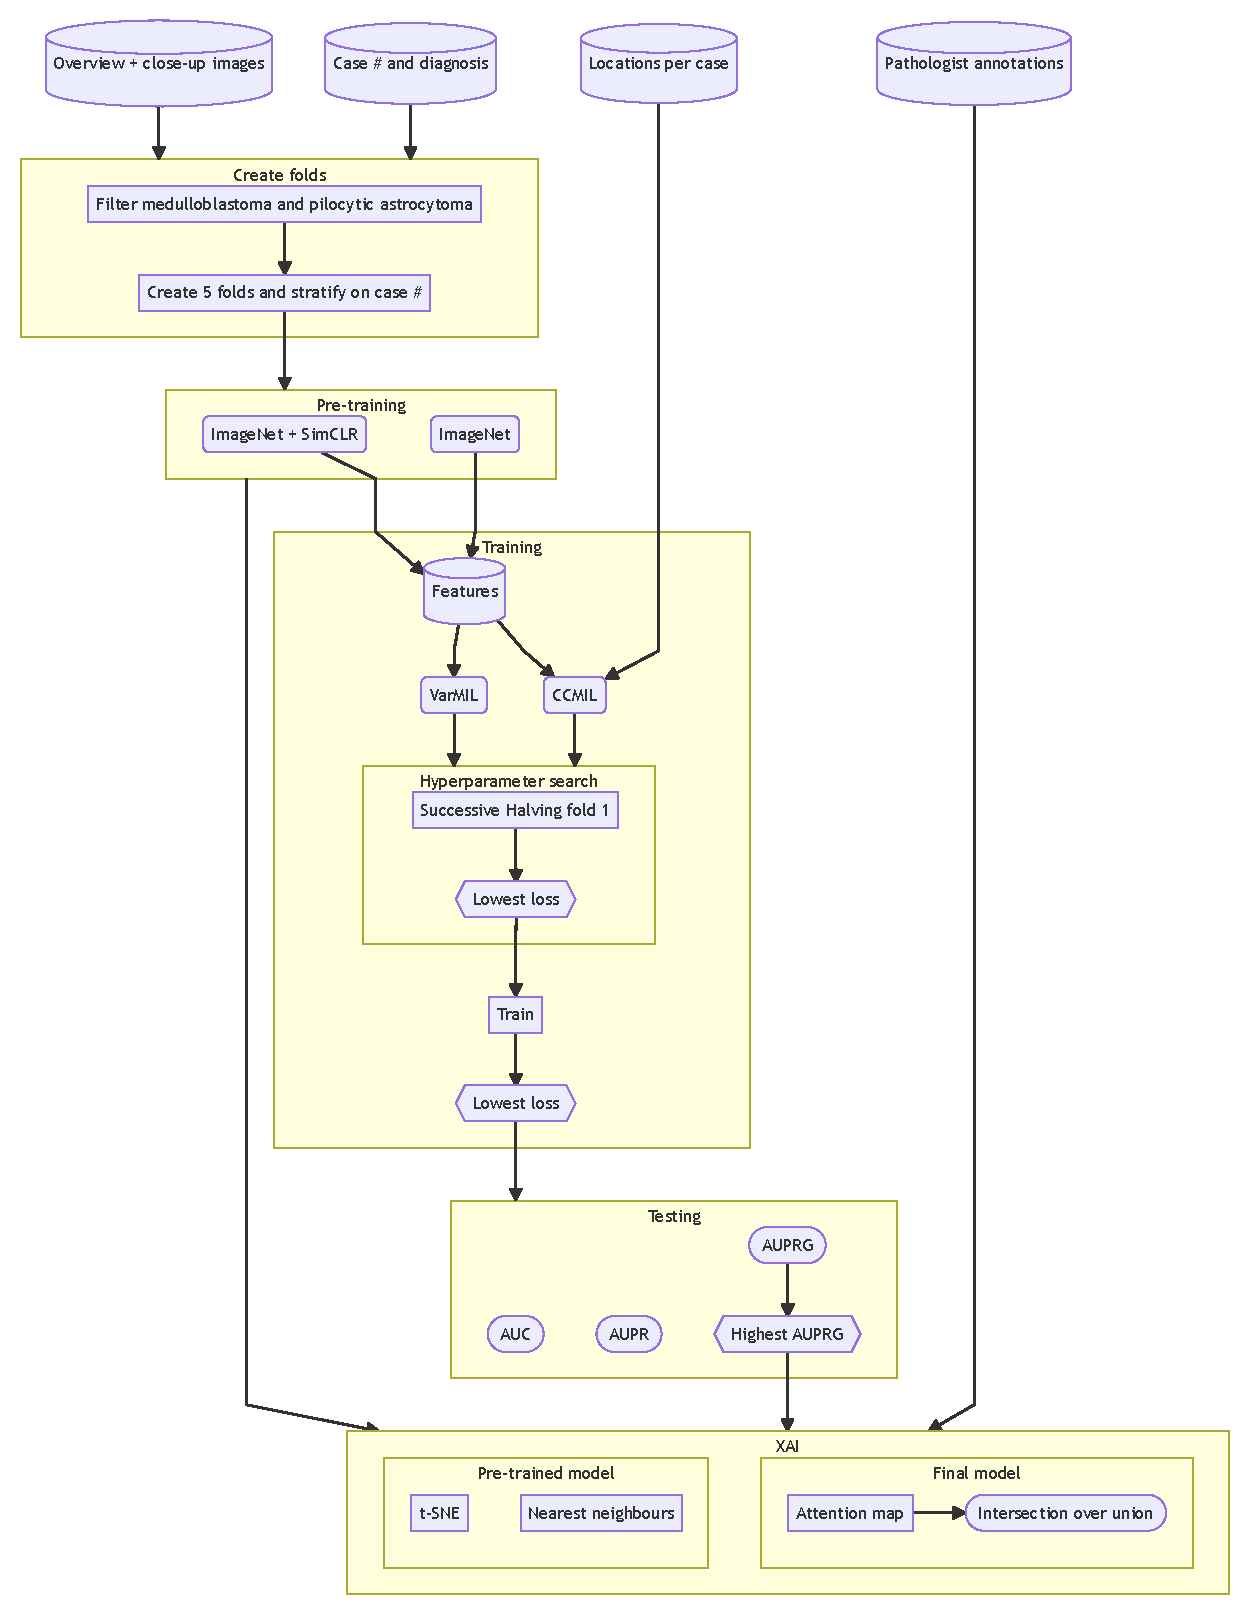
\includegraphics[width=\linewidth]{mermaid/brain/analytical-methods.pdf}
    \caption[Flowchart of training SCLICOM.]{
        Flowchart for training of Self-supervised pre-training and CLInical COntext-aware Multi-instance learning (SCLICOM).
        The images are filtered by diagnosis and divided in five folds.
        An ImageNet initialized SimCLR model is trained.
        From this model and an ImageNet initialized model, features are extracted.
        The extracted features are used to train VarMIL and CCMIL models.
        One fold for every model is used to search for hyperparameters with which the models are further trained.
        The models are tested on the test set and AUC, AUPR, and AUPRG are reported.
        Attention maps are made from the best performing model and compared with pathologist annotations.
    }
    \label{fig:flowchart-sclicom}
\end{figure*}

The model consists of two stages: the feature extractor and the classifier.
They are trained separately.

\subsubsection{Feature extractor}
The feature extractor is a convolutional neural network with a ShuffleNetV2 (x1.0)~\sidecite{Ma2018} backbone, provided by imgclsmob~\sidecite{imgclsmob2023}, outputting a vector with length 1024.
Two backbones were used as feature extractor.
One was pre-trained on ImageNet and another feature extractor has an He initialized ShuffleNetV2 backbone and was trained using SimCLR.
The SimCLR projection head consisted of two linear layers with dimensions 1024 and 128.

\subsubsection{Classifier}
The classifier is a MIL model applied to the features extracted by the pretrained feature extractor.
DeepMIL, VarMIL and CCMIL are used as classifiers.
For DeepMIL, the attention block consists of a linear layer of size 256 with dropout and a $\tanh$ activation function and another linear layer with dropout, resulting in a scalar.
The classifier block consists of a linear layer with dropout and $\mathrm{softmax}$ activation function and has an output size of the number of classes to predict, \ie two.
For VarMIL, the last linear layer accepts an input of twice the size, to account for the variance vector.
For CCMIL, the last linear layer maps textual tumor locations (\eg "fourth ventricle") to a 312-dimensional space.
Text is embedded with TinyClinicalBERT~\sidecite{Rohanian2023}, provided by Huggingface Transformers~\sidecite{Wolf2020}, using its \texttt{[CLS]}-token.
During training, BERT's parameters were frozen.
All other parameters were He initialized.
To validate BERT, the location embeddings were projected to two dimensions with t-SNE.

\subsubsection{Internal validation}\label{subsubsec:slicom-folds}
The data was split in five training and test data folds, stratified by case.
All training splits were further split randomly, again stratified by case.
The flow of images to splits is visualized in \cref{app:folds-splits-viz}.

\subsubsection{Pre-training}
The latter model is trained on 1 NVIDIA A30 GPU for 2 days with a bag size of 256 with gradients accumulated over two epochs to imitate larger bags.
The Adam optimizer was used with a learning rate of $3\times 10^{-4}$ and $\beta_{1,2} = \{0.9,\, 0.999\}$ without weight decay and without a learning rate scheduler.

The pretrained models are internally assessed by visualizing the extracted features in two ways.
First, tiles corresponding to ten nearest neighbors in feature space are compared.
Second, the features are projected with two-dimensional t-SNE after extracting the ten principal components with PCA.
The t-SNE projections are colored by image and case identifier, and diagnosis.

\subsubsection{Training}
In total, 15 models are trained using PyTorch Lightning~\sidecite{Falcon2019}: 3 model definitions on 5 folds.
For every fold and model a Successive Halving hyperparameter search is performed on 1 NVIDIA A100 GPU partitioned in 8 for a minimum of 30 epochs and a maximum of 500 epochs with resources managed by Ray Tune~\sidecite{Liaw2018} and 100 trials suggested by a grouped multivariate TPE sampler provided by Optuna~\sidecite{Akiba2019}.
See \cref{tab:hyperparameter_search_space} for the hyperparameter search space.
Using the configuration that lead to the model with the lowest validation loss is used for training on all splits for 2000 epochs.
The models were trained on 1 NVIDIA A100 GPU for 2 hours with a bag size of 1, \ie all tiles from one image at a time.
The learning rate was varied with the cosine annealing scheduler.

\begin{margintable}
    \caption[Hyperparameter search space]{
        Hyperparameter search space with dropout, learning rate, momentum and weight decay.
    }
    \label{tab:hyperparameter_search_space}
    \begin{tabular}{lcc}
        \toprule
        Parameter &  Min. & Max. \\
        \midrule
        Dropout & 0 & 1 \\
        Learning rate & $10^{-5}$ & $10^{-2}$ \\
        Momentum & 0 & 1 \\
        Weight decay & $10^{-4}$ & 1 \\
        \bottomrule
    \end{tabular}
\end{margintable}

\subsubsection{Testing}
All models from the same initialization were evaluated against a test set.
Performance is visualized using an ROC, PR and PRG curve.
AUC, AUPR, and AUPRG with their \qty{95}{\percent} confidence interval are reported to compare models.
Metrics were calculated by Torchmetrics~\sidecite{Detlefsen2022} and pyprg~\sidecite{Flach2015}.

\subsubsection{Attention maps}
To verify and to gain knowledge of the inner workings of the model, attention maps are created.
The attention maps are acquired by multiplying the min-max-normalized attention weights with their corresponding tiles.
The maps are compared with tumor annotations from a pathologist.
The IoU of the tumor is reported.
